  \chapter{Binomial Filter}
   Binomial filters are simple and efficient structures based on the binomial coefficients for implementing Gaussian filtering. 
   To extract these coefficients, we could use Pascal's Triangle.\\
   The rows of Pascal's triangle are conventionally enumerated starting with row $ n = 0 $ at the top (the 0\^{th} row). The entries in each row are numbered from the left beginning with $ k = 0 $ and are usually staggered relative to the numbers in the adjacent rows. The triangle may be constructed in the following manner: In row $ 0 $ (the topmost row), there is a unique nonzero entry$  1 $. Each entry of each subsequent row is constructed by adding the number above and to the left with the number above and to the right, treating blank entries as $  0 $. For example, the initial number in the first (or any other) row is $ 1  $(the sum of $ 0 $ and $ 1 $), whereas the numbers $ 1 $ and $ 3 $ in the third row are added to produce the number $ 4 $ in the fourth row.
   \bigskip
\begin{center}
	  \begin{tabular}{>{$n=}l<{$\hspace{15pt}}*{13}{c}}
  	0 &&&&&&&1&&&&&&\\    1 &&&&&&1&&1&&&&&\\    2 &&&&&1&&2&&1&&&&\\    3 &&&&1&&3&&3&&1&&&\\    4 &&&1&&4&&6&&4&&1&&\\    5 &&1&&5&&10&&10&&5&&1&\\    6 &1&&6&&15&&20&&15&&6&&1
  \end{tabular}
\end{center}
\bigskip
The first  odd sized serie is:
 \begin{center}
	1 \quad 2 \quad 1\\
\end{center}
 this form the basis for the 3x3 binomial filter. \\
 The weights of the binomial filter are biggest at the center and taper down towards the outer areas of the neighborhood. \\ 
 To create the 2D low pass binomial filter, we have to form the outer product of the row with its corresponding column. In simple terms take the row and multiply each element in it by the first value in the row. Then take the row and multiply each element in it by the second value in the row. Repeat this until we have multiplied the row by every element in the row. Then stack each of these resulting rows to make a square table or matrix. \\
 For example, the 3x3 matrix is generated as 
   \begin{center}
   	$ \begin{bmatrix}1\\ 2 \\ 1 \end{bmatrix} \cdot
   	\begin{bmatrix} 1 & 2 & 1 \end{bmatrix}= \begin{bmatrix}1 & 2 & 1\\
   	2 & 4 & 2   	\\1 & 2 & 1\end{bmatrix}$
   \end{center}
      After multipling, we need to normalize, so the overall 3x3 binomial filter is:
   \begin{center}
   	$   \dfrac{1}{16}\begin{bmatrix}1 & 2 & 1\\
   	2 & 4 & 2   	\\1 & 2 & 1\end{bmatrix}$
   \end{center}
    In particular, given a cell in position $ (x, y) $, the final value of the computation should be:
   
     \begin{equation} \label{eq:BN eq}
     \begin{aligned}
     f(x,y)= \dfrac{1}{16} & [  1(x-1,y-1) + 2(x-1,y)+ 1(x-1, y+1)+\\
     & + 2(x,y-1) + 4(x,y)+ 2(x, y+1)+\\
     & + 1(x+1,y-1) + 2(x+1,y) + 1(x+1, y + 1) ] \\
     \end{aligned}
     \end{equation}
     
     As shown in the figure below, the value of the dark blue rectangle can be calculated as the weighted mean of all the light blue rectangles:
       
        \begin{figure}[h!]
        	\centering
        	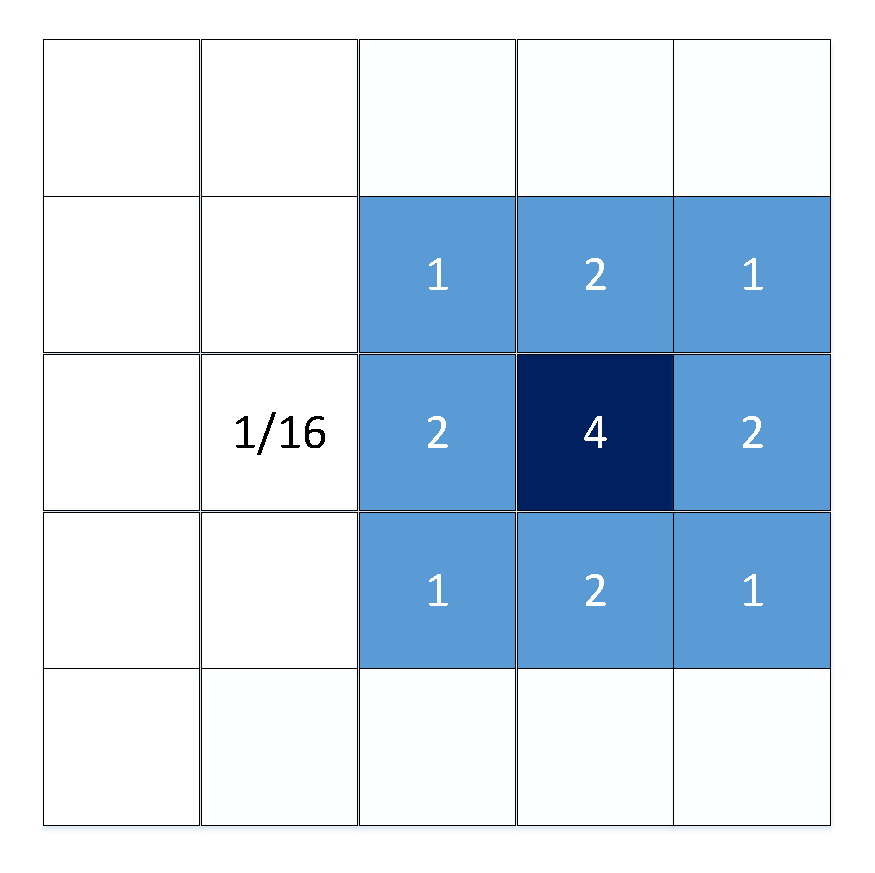
\includegraphics[width=\textwidth]{imm/bf/bf1.pdf} 	\caption{Binomial Filter for a generic cell} 
        	\label{fig:bf1}
        \end{figure}
        \clearpage
        \section{Hardware implementations} \label{bfh}
        \subsection{Hardware implementation type 1} \label{h1}
        This implementation will focus only to the possible cells for the binomial filter, i.e. the ones not in the border of the matrix, bevause they are leaved unchanged.
        \begin{enumerate}
        	\item for each row, whenever we find three consecutive cells, we evaluate the sum \begin{center}
        		$ S_{x,y}=cell_{x-1,y}+2\cdot cell_{x,y}+cell_{x+1,y}$
        	\end{center}
        	In order to so, we need 2 adder: we shift by one position the value of the central cell (i.e. multiply by two) and sum it with the left and the right cells as shown in fig \ref{fig:bflev11} while fig \ref{fig:bflev1} shows the overall picture of this step.
        	\begin{figure}[h!]
        		\centering
        		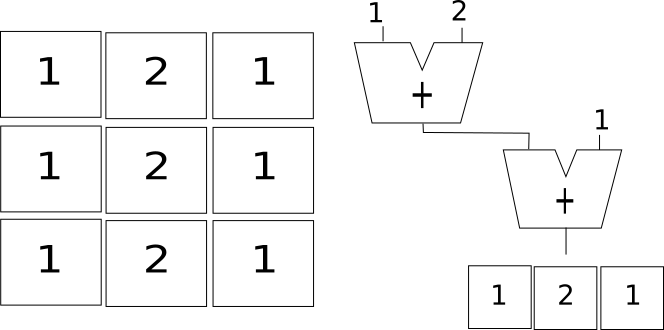
\includegraphics[width=\textwidth]{imm/bf/bflev11.png}  
        		\caption{Weighted sum for three consecutive cells} 
        		\label{fig:bflev11}
        			\end{figure}
        			
        	\begin{figure}[h!]
        		\centering
        		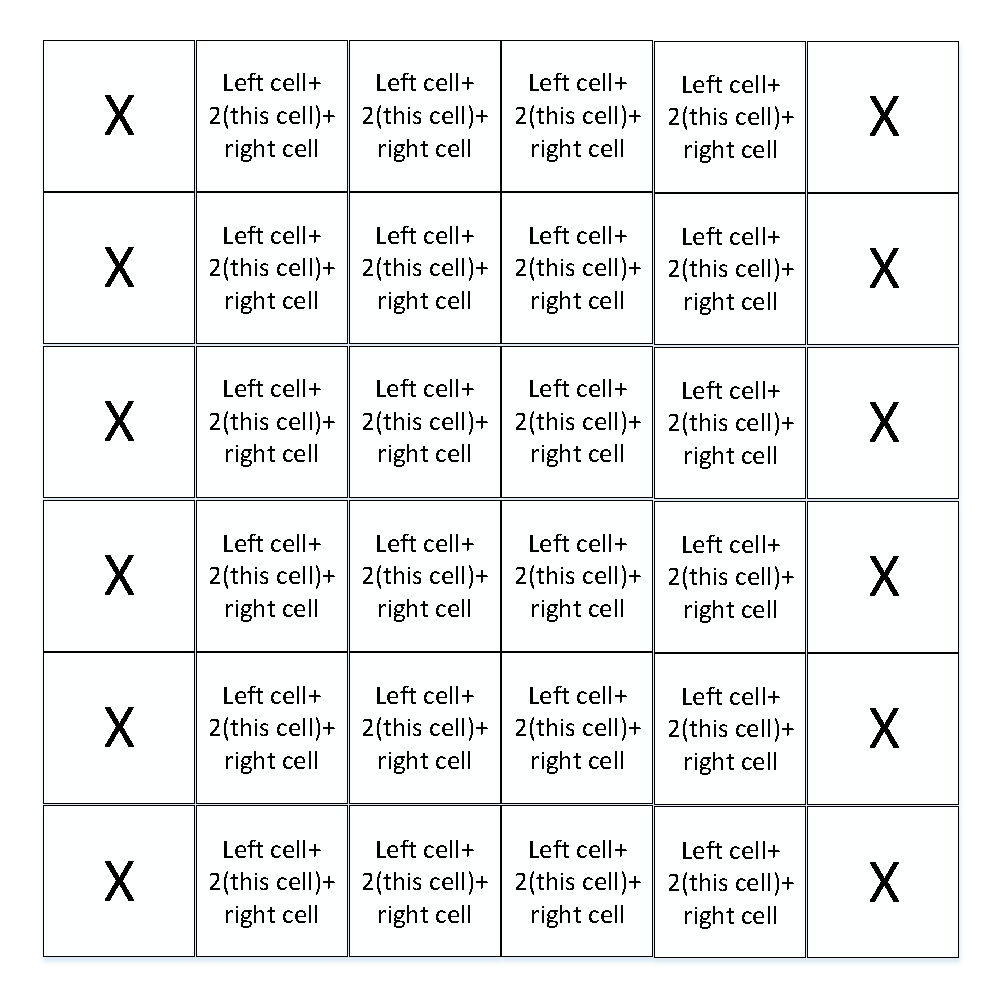
\includegraphics[width=\textwidth]{imm/bf/bflevel1.pdf}  
        		\caption{First part of the binomial filter HW implementation} 
        		\label{fig:bflev1}
        	\end{figure}
        	\clearpage
        	\item Taking the result of the previous step as a matrix, for each column whenever we found three consecutive cells we evaluate the sum
        	\begin{center}
        			$ SUM_{x,y}=S_{x,y-1}+2\cdot S_{x,y}+S_{x,y+1}$
        	\end{center}
        	which is equal to 
        	\begin{equation} \label{eq:BF_eq}
        	\begin{aligned}
        SUM_{x,y} =& (cell_{x-1,y-1}+2\cdot cell_{x,y-1}+cell_{x+1,y-1})+\\
        & +2\cdot (cell_{x-1,y}+2\cdot cell_{x,y}+cell_{x+1,y})+\\
        &+(cell_{x-1,y+1}+2\cdot cell_{x,y+1}+cell_{x+1,y+1}) =\\
        =& cell_{x-1,y-1}+2\cdot cell_{x,y-1}+cell_{x+1,y-1}+\\
        &+ 2\cdot cell_{x-1,y}+4\cdot cell_{x,y}+2\cdot cell_{x+1,y}+\\
        &+ cell_{x-1,y+1}+2\cdot cell_{x,y+1}+cell_{x+1,y+1}
        	\end{aligned}
        	\end{equation}
        	fig \ref{fig:bflev12} shows this step
        	\bigskip
       	\begin{figure}[h!]
       		\centering
       		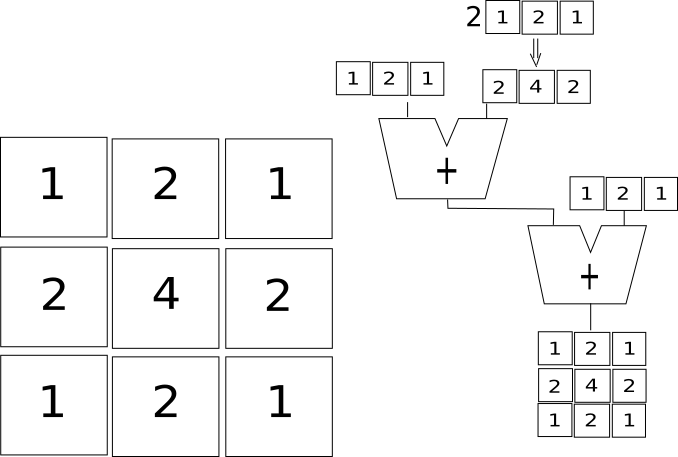
\includegraphics[width=0.95\textwidth]{imm/bf/bflev12.png}  
       		\caption{Weighted sum for 3x3 cells} 
       		\label{fig:bflev12} 	
        \end{figure}
        	\begin{figure}[h!]
        		\centering
        		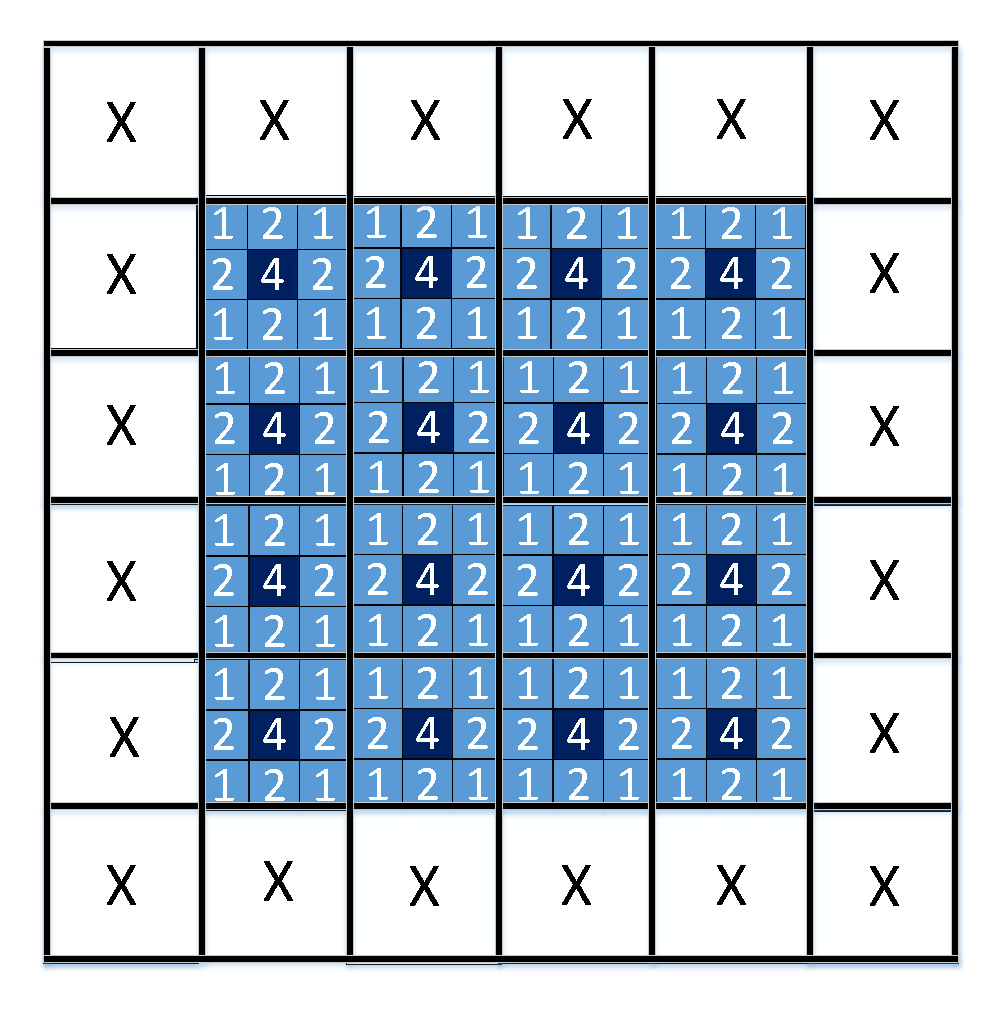
\includegraphics[width=\textwidth]{imm/bf/bflev2.pdf}  
        		\caption{Weighted sum for all 3x3 cells} 
        		\label{fig:bflev2}
        	\end{figure}
        \item Now that we have the weighted sum for all the 3x3 cells, we have to divided by 16. In order to do so, the quickest way is to shift the result by 4 bits.
        The values of the cells in the border of the matrix, are unchanged in the final result.
        	\end{enumerate}
     \clearpage
     \subsection{Hardware implementation type 2} \label{h2}
     This implementation will focus to all the cells. 
     The only difference between this implementation and the one  described in the subsection \ref{h1} is that now we apply the Binomial Filter also for the cells in the border of the matrix.
     We take the original matrix and we set a neighborhood of cells at $ '0' $ as shown in fig \ref{fig:h2} where the original matrix has benn highlighted in black.
     The procedure to evaluate the final result of the binomial filter is the same as explained in the subsection  \ref{h1}.
      \begin{figure}[h!]
      	\centering	
      	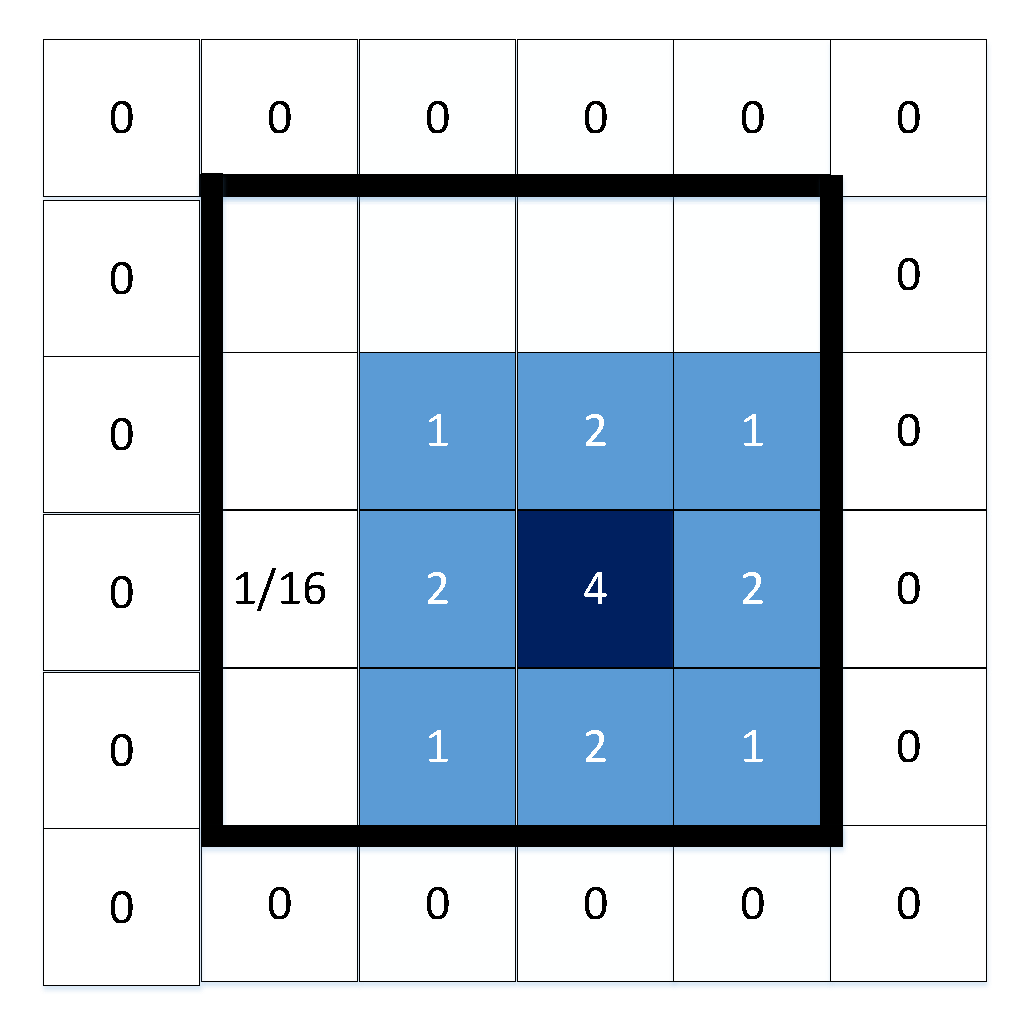
\includegraphics[width=0.9\textwidth]{imm/bf/bf_h2.pdf}  
      	\caption{Binomial Filter, second implemetation} 
      	\label{fig:fig:h2}
      \end{figure} 
     \section{Simulations}   
     \subsection{Simulation type 1} \label{sim1}
     The simulation shown in this work is referred to the hardware implementation descrived in the subsection \ref{h1} where the values of the matrix's border are leaved unchanged.
     In this testbench, we have a matrix 4x4 (fig.\ref{fig:tb_bf} highlighted in yellow, and the output highlighted in red).
    
     
     \begin{figure}[h!]
     	\centering	
     	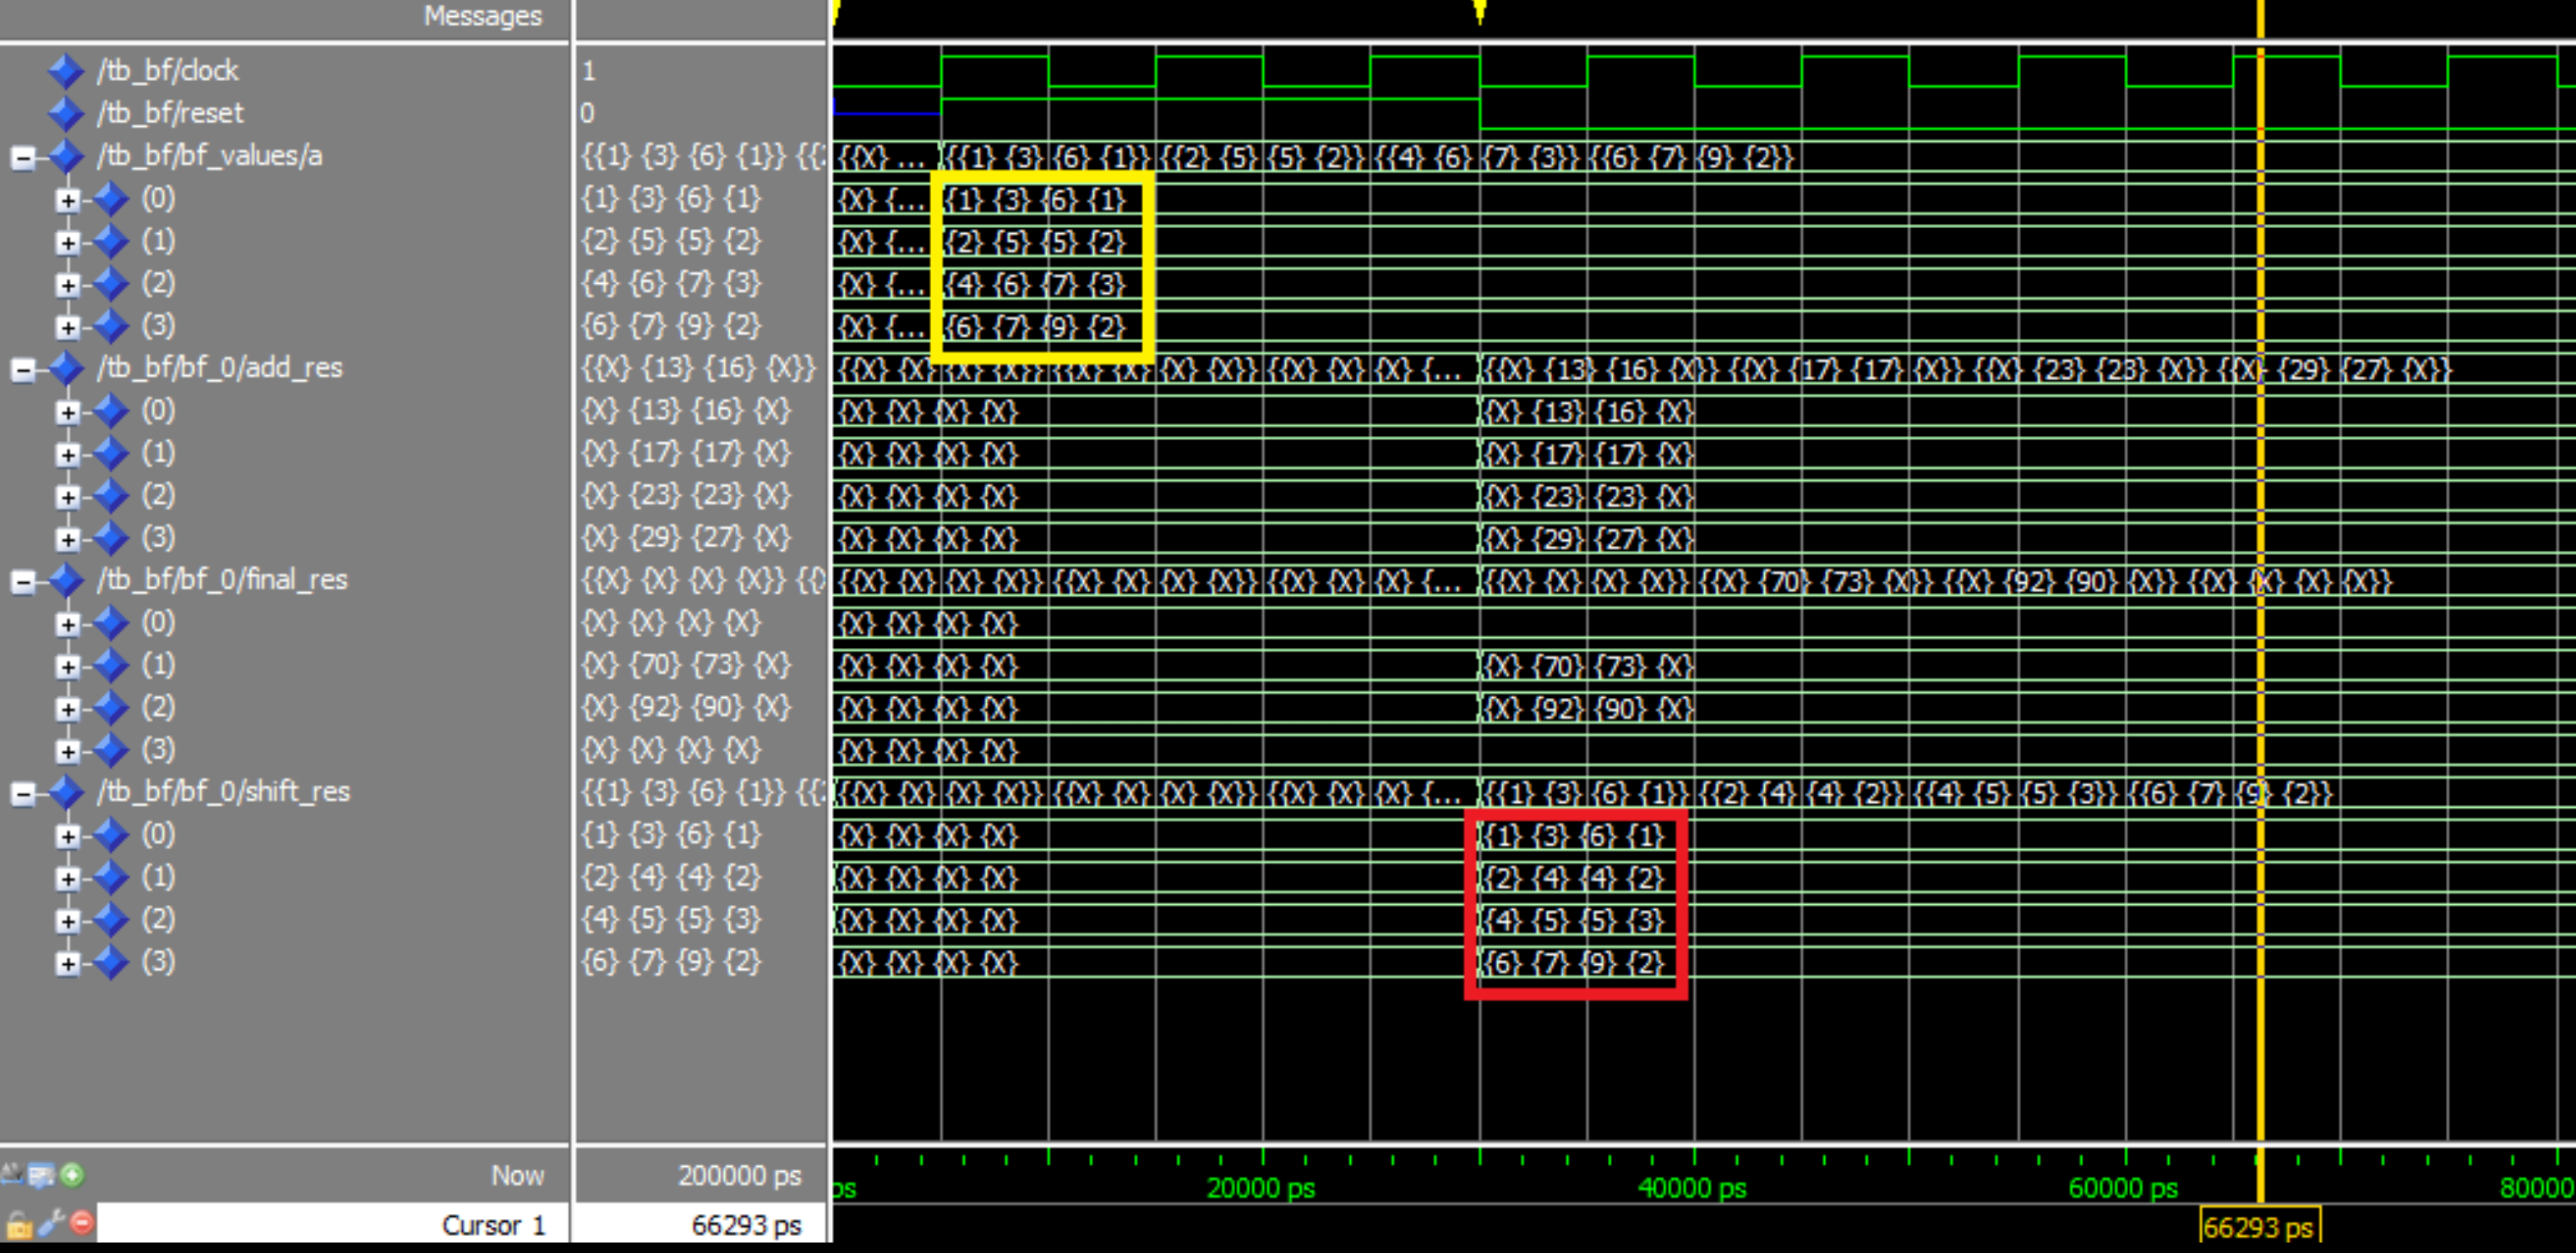
\includegraphics[width=\textwidth]{imm/bf/tb_bf.png}  
     	\caption{Binomial Filter-Results of the simulation type 1} 
     	\label{fig:tb_bf}
     \end{figure}
     
     At the beginning we have an input array that contains the values of the matrix   \begin{center}
     	$ \begin{bmatrix}
     	1 & 3 & 6 & 1\\
	     	2 & 5 & 5 & 2   	\\
	     	4&6 & 7 & 3\\
	     	6&7 & 9 & 2
	     	\end{bmatrix}$
	     	     \end{center}
	  The first step of this implementation is to do the partial weighted sum for three consecutive cell
	  \begin{center}
	  	$ S_{x,y}=cell_{x-1,y}+2\cdot cell_{x,y}+cell_{x+1,y}$\\
	  	$  \forall x\in [1,n-2] \quad\forall y\in[0,n-1]$
	  \end{center}
	   \begin{center}
	   	$ \begin{bmatrix}
	   	X\quad & 1+2\cdot3+6 \quad& 3+2\cdot6+1\quad & X\\
	   	X\quad & 2+2\cdot5+5 \quad& 5+2\cdot5+2\quad & X   	\\
	   	X\quad&4+2\cdot6+7 \quad& 6+2\cdot7+3\quad & X\\
	   	X\quad&6+2\cdot7+9 \quad& 7+2\cdot9+2\quad & X
	   	\end{bmatrix}$
	   \end{center}
	   which will lead us to the result
	   \begin{center}
	   	$ \begin{bmatrix}
	   		X & 13 & 16 & X\\
	   		X & 17 & 17 & X   	\\
	   		X&23 & 23 & X\\
	   		X&29 & 27 & X
	   	\end{bmatrix} $
	   \end{center}
	   which is the same shown in the simulation (fig \ref{fig:tb_bf}, \textit{add\_res} array).\\
	    Now we have to do the final sum
	   \begin{center}
	   	$ SUM_{x,y}=S_{x,y-1}+2\cdot S_{x,y}+S_{x,y+1}$\\
	   		$  \forall x\in [1,n-2] \quad\forall y\in [1,n-2] $
	   \end{center}
	   \bigskip
	  \begin{center}
	  	$ \begin{bmatrix}
	  	X & X & X & X\\
	  	X \quad& 13+2\cdot17+23\quad & 16+2\cdot17+23 \quad& X   	\\
	  	X\quad&17+2\cdot23+29 \quad& 17+2\cdot23+27 \quad& X\\
	  	X&X & X & X
	  	\end{bmatrix} = \begin{bmatrix}
	  	X & X & X & X\\
	  	X & 70 & 73 & X   	\\
	  	X&92 & 90 & X\\
	  	X&X & X & X
	  	\end{bmatrix}$
	  \end{center}
	  this matrix is the same we obtained in the simulation (fig \ref{fig:tb_bf}, \textit{final\_res} array).
	  The work is not over yet because we need to divide these sums by 16
	  \begin{center}
	  	$ \begin{bmatrix}
	  	X & X & X & X\\
	  	X & \frac{70}{16} & \frac{73}{16} & X   	\\
	  	X&\frac{92}{16}  & \frac{90}{16}  & X\\
	  	X&X & X & X
	  \end{bmatrix}=\begin{bmatrix}
	  X & X & X & X\\
	  X & 4.375 & 4.5625 & X   	\\
	  X&5.75  & 5.625  & X\\
	  X&X & X & X
	  \end{bmatrix}$
	  \end{center}
	  Since the values of the pixel are integer, we can round the matrix as\begin{center}
	  	$ 
	  \begin{bmatrix}
	  	X & X & X & X\\
	  	X & 4 & 4 & X   	\\
	  	X&5  & 5  & X\\
	  	X&X & X & X
	  \end{bmatrix}$
	  \end{center}
	  so the final result is \begin{center}
	  	$ 
	  	\begin{bmatrix}
	  	1 & 3 & 6 & 1\\
	  	2 & 4 & 4 & 2   	\\
	  4&5  & 5  & 3\\
	  	6&7 & 9 & 2
	  	\end{bmatrix}$
	  \end{center}
	  which is the same as shown in the simulation (fig \ref{fig:tb_bf}, \textit{shifft\_res} array).
	  \subsection{Simulation type 2}
	
	  The simulation shown in this work is referred to the hardware implementation descrived in the subsection \ref{h2} where also the final values of the matrix's border are computed using the binomial filter criteria.
	  In this testbench, we have a matrix 4x4 (fig.\ref{fig:tb_bf} highlighted in yellow, and the output highlighted in red).
	  
	  
	  \begin{figure}[h!]
	  	\centering	
	  	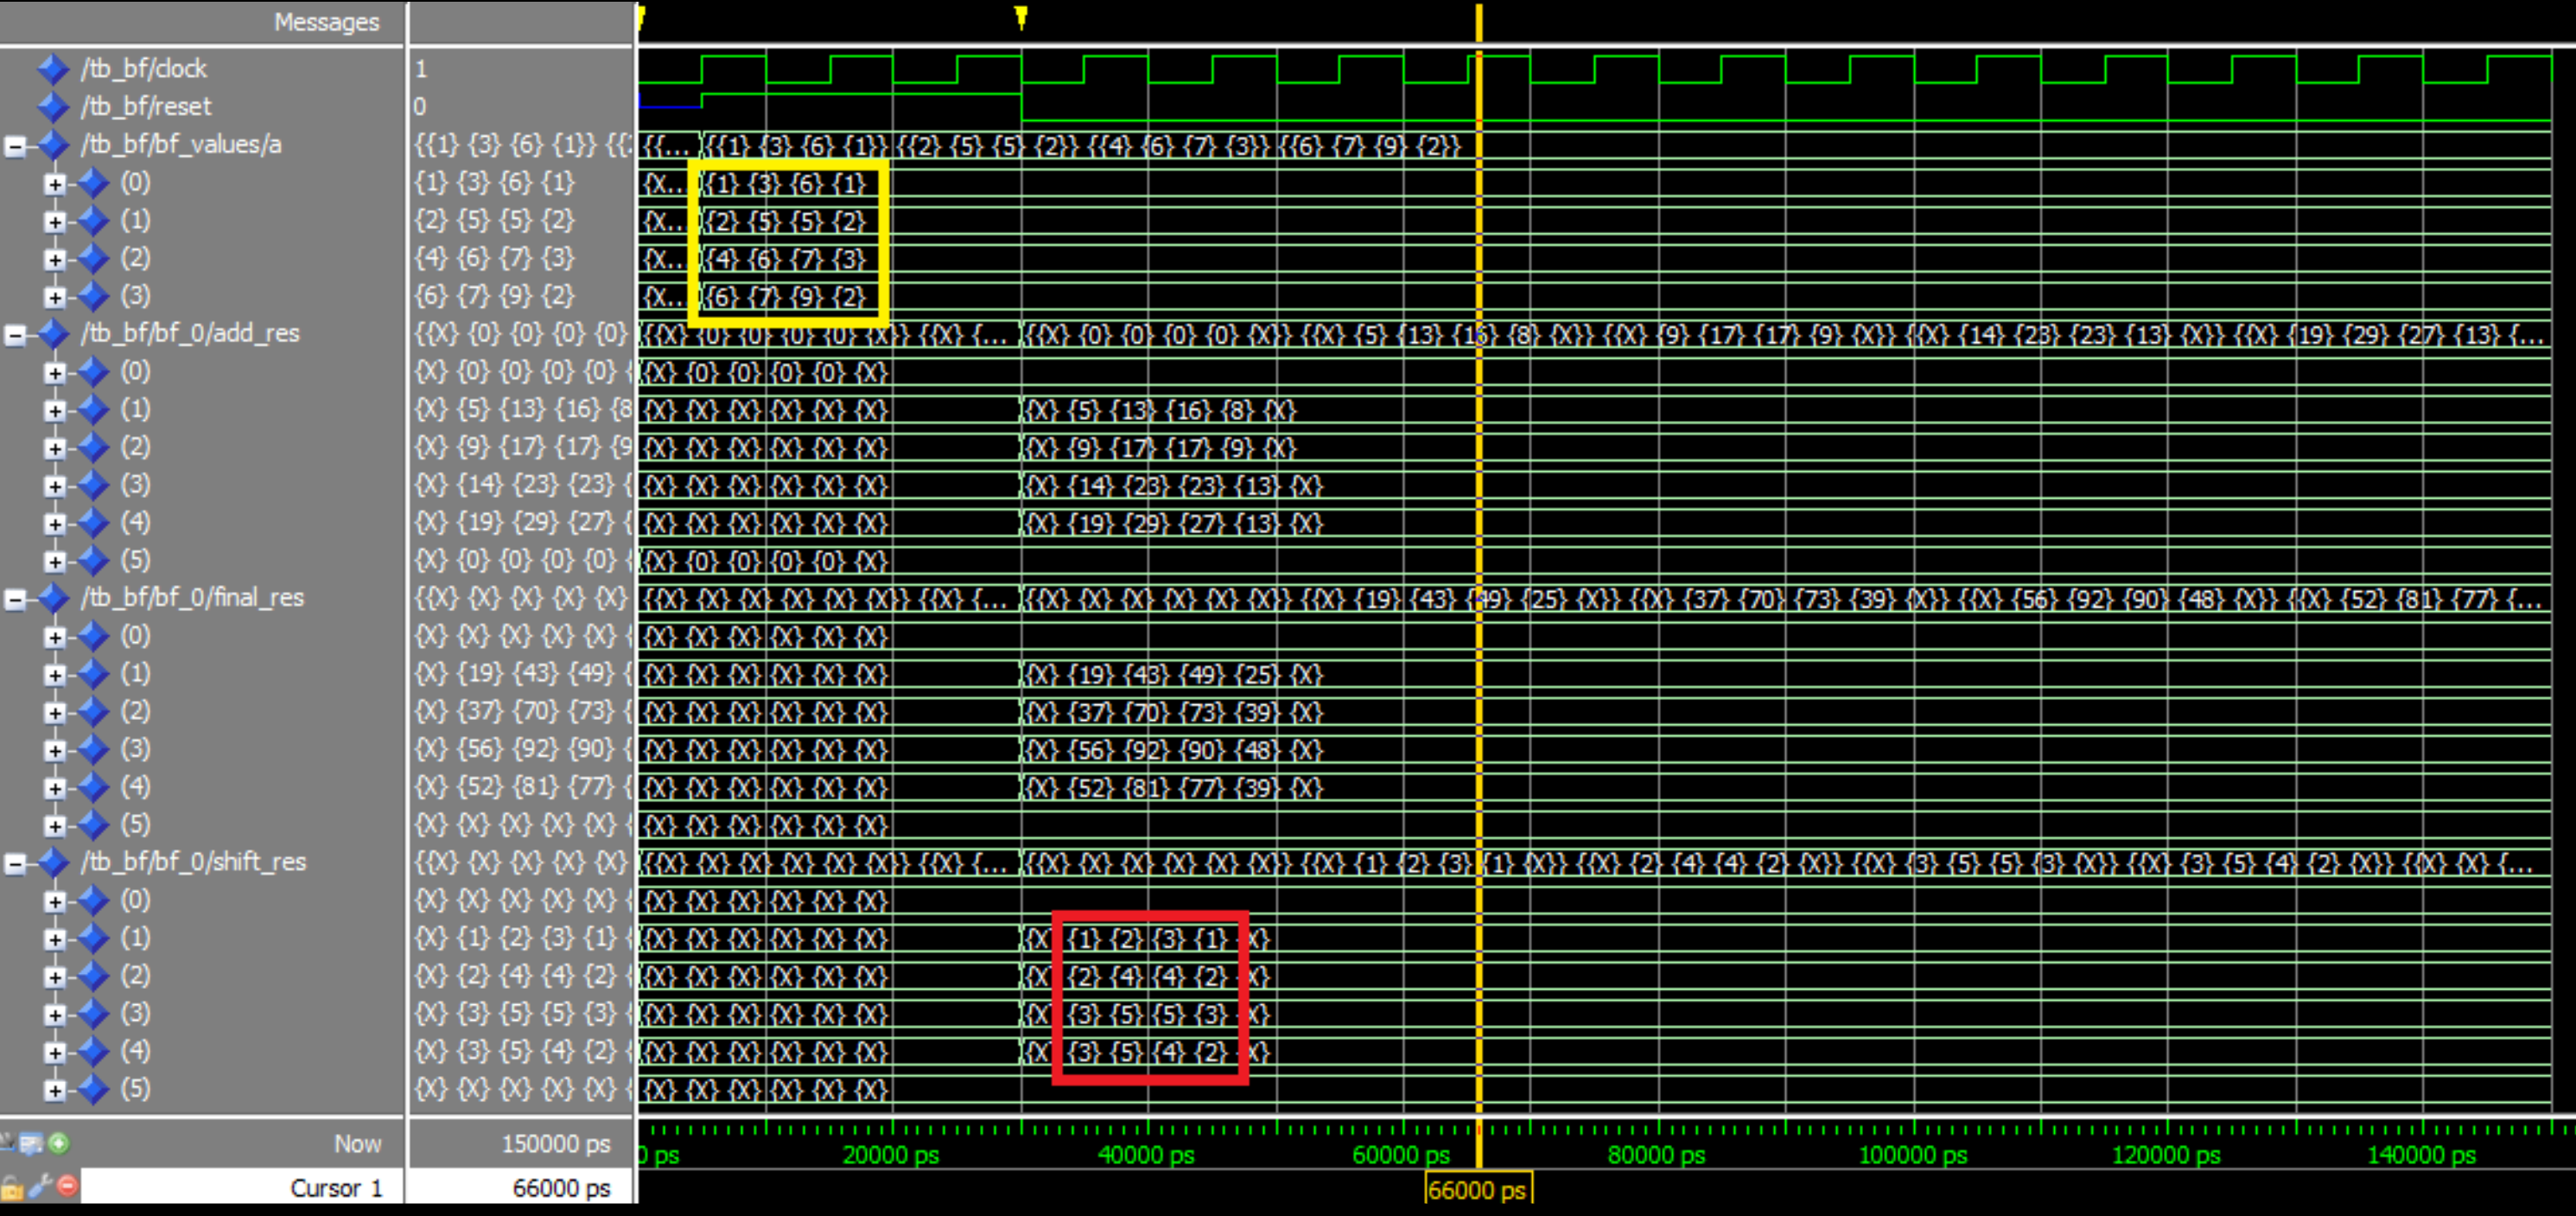
\includegraphics[width=\textwidth]{imm/bf/bfwavev2.png}  
	  	\caption{Binomial Filter-Results of the simulation type 2} 
	  	\label{fig:tb_bf2}
	  	\end{figure}
	At the beginning we have an input array that contains the values of the matrix   \begin{center}
		$ \begin{bmatrix}
		1 & 3 & 6 & 1\\
		2 & 5 & 5 & 2   	\\
		4&6 & 7 & 3\\
		6&7 & 9 & 2
		\end{bmatrix}$
	\end{center}
	For this implementation, we will perform the binomial filter for the matrix that has a border of  $ '0' $ and in the center the input matrix.
	 \begin{center}
	 	$ \begin{bmatrix}
	 	0&0 &0  &0  & 0&0\\
	 	0&1 & 3 & 6 & 1&0\\
	 	0&2 & 5 & 5 & 2  &0 	\\
	 0&	4&6 & 7 & 3&0\\
	 0&	6&7 & 9 & 2&0\\
	 	0&0 &0  &0  & 0&0
	 	\end{bmatrix}$
	 	 \end{center}
Now we perform the same steps described in section \ref{sim1}.	
We do the partial weighted sum for three consecutive cell
\begin{center}
	$ S_{x,y}=cell_{x-1,y}+2\cdot cell_{x,y}+cell_{x+1,y}$\\
	$  \forall x\in [1,n-2] \quad\forall y\in[0,n-1]$
\end{center} 	 
	\begin{center}
		$ \begin{bmatrix}
		X&0&0&0&0&X\\
		X\quad&2\cdot1+3\quad & 1+2\cdot3+6 \quad& 3+2\cdot6+1\quad & 6+2\cdot1\quad&X\\
		X\quad&2\cdot2+5\quad & 2+2\cdot5+5 \quad& 5+2\cdot5+2\quad & 5+2\cdot2  \quad&X 	\\
		X\quad&2\cdot4+6\quad&4+2\cdot6+7 \quad& 6+2\cdot7+3\quad & 7+2\cdot3\quad&X\\
		X\quad&2\cdot6+7\quad&6+2\cdot7+9 \quad& 7+2\cdot9+2\quad & 9+2\cdot2\quad&X\\
		X&0&0&0&0&X
		\end{bmatrix}$
	\end{center}
	which will lead us to the result
	\begin{center}
		$ \begin{bmatrix}
		X&0&0&0&0&X\\
		X\quad&5\quad & 13 \quad& 16\quad & 8\quad&X\\
		X\quad&9\quad &17 \quad& 17\quad & 9  \quad&X 	\\
		X\quad&14\quad&23 \quad&23\quad & 13\quad&X\\
		X\quad&19\quad&29 \quad& 27\quad & 13\quad&X\\
		X&0&0&0&0&X
		\end{bmatrix}$
	\end{center}
	which is the same shown in the simulation (fig \ref{fig:tb_bf2}, \textit{add\_res} array).\\ 	 
	  	Now we have to do the final sum
	  	\begin{center}
	  		$ SUM_{x,y}=S_{x,y-1}+2\cdot S_{x,y}+S_{x,y+1}$\\
	  		$  \forall x\in [1,n-2] \quad\forall y\in [1,n-2] $
	  	\end{center}
	  	\bigskip
	  	\begin{center}
	  		$ \begin{bmatrix}
	  		X & X & X & X &X&X\\
	  		X\quad & 2\cdot5+9\quad& 2\cdot13+17\quad&2\cdot16+17\quad&2\cdot8+9\quad&X\\
	  		X \quad&5+2\cdot9+17\quad& 13+2\cdot17+23\quad & 16+2\cdot17+23 \quad& 8+2\cdot9+13\quad&X   	\\
	  		X\quad&9+2\cdot14+19\quad&17+2\cdot23+29 \quad& 17+2\cdot23+27 \quad& 9+2\cdot13+13\quad&X\\
	  		X\quad & 14+2\cdot19\quad& 23+2\cdot29\quad&23+2\cdot27\quad&13+2\cdot13\quad&X\\
	  		X&X & X & X &X&X
	  		\end{bmatrix} = $
	  		\bigskip$=\begin{bmatrix}
	  	X & X & X & X &X&X\\
	  	x & 19 & 43 & 49 & 25 & X\\
	  	X & 37 &70 & 73 & 39 & X   	\\
	  		X&56 & 92 & 90 & 48& X\\
	  		X&52&81&77&39&X\\
	  		X & X & X & X &X&X
	  		\end{bmatrix}$
	  	\end{center}
	  	this matrix is the same we obtained in the simulation (fig \ref{fig:tb_bf2}, \textit{final\_res} array).
	  	The work is not over yet because we need to divide these sums by 16\\
	  	\begin{center}
	  	$	\begin{bmatrix}
  			X & X & X & X &X&X\\
  			X & \frac{19}{16} & \frac{43}{16} & \frac{49}{16} & \frac{25}{16} & X\\
  			X & \frac{37}{16} &\frac{70}{16} & \frac{73}{16} & \frac{39}{16} & X   	\\
  			X&\frac{56}{16} & \frac{92}{16} & \frac{90 }{16}& \frac{48}{16}& X\\
  			X&\frac{52}{16}&\frac{81}{16}&\frac{77}{16}&\frac{39}{16}&X\\
  			X & X & X & X &X&X
	  		\end{bmatrix}=	\begin{bmatrix}
	  		X & X & X & X &X&X\\
	  		X & 1.1875 & 2.6875 & 3.0625 & 1.5625 & X\\
	  		X & 2.3125 &4.375 & 4.5625 & 2.4375 & X   	\\
	  		X&3.5 & 5.75 & 5.625& 3& X\\
	  		X&3.25&5.0625&4.8125&2.4375&X\\
	  		X & X & X & X &X&X
	  		\end{bmatrix}$
	  	\end{center}\bigskip
	  	Since the values of the pixel are integer, we can round the matrix as\\
	  	\begin{center}
	  		$	\begin{bmatrix}
	  		X & X & X & X &X&X\\
	  		X & 1 & 2 & 3 & 1 & X\\
	  		X & 2 &4 & 4 & 2 & X   	\\
	  		X&3 & 5 & 5& 3& X\\
	  		X&3&5&4&2&X\\
	  		X & X & X & X &X&X
	  		\end{bmatrix}$
	  		\end{center}
	  	
	  \section{Comparison}
	  \subsubsection{Logic-In-Memory implementation}
	  The architecture of the Logic-In-memory was already explained in the subsection \ref{sssec:1}.
	  The pseudocode for the LIM is
	  \begin{enumerate}
	  	\item Each cell reads its own value;
	  	\item Reads all neighbouring cells data (8 different values); 
	  	\item Sums all values and divides them by 16;
	  	\item Writes the final result in its own memory;
	  \end{enumerate}
	 The main advantage of the LIM architecture is the parallelism: the presence of many cells that can work autonomously greatly increases the speed of the computation of algorithms that can be executed in parallel.
	 It has been calculated that the total duration for the computation is equal to: 
	 \begin{itemize}
	 	\item N clock cycles to write the data;
	 	\item 28 clock cycles to compute the algorithm;
	 	\item 2N+1 clock cycles to read the data through a remote read. Therefore,
	 \end{itemize}   \begin{center}
	 	 $ t = N + 28 + 2N +1=3N + 29 $
	\end{center}
	
	 \begin{center}
	 	\begin{tabular}{ | p{1.7cm} | c | c | c |}
	 			
	 		\hline
	 	 & LIM & This work & This work\\
	 	\label{table:bf_tab}	& & version 1& version 2\\
	 			 		\hline
	 		Area & $ N\cdotp N $ cells  &  $ 2N\cdotp (N-2)+$& $(4N-4)+$ \\
	 		& & $+2(N-2)^2$ adders & $2(N-2)^2$ adders \\
	 		\hline
	 		Time & $ 3N + 29 $ cycles
	 		&
	 		 time for 4 adders  &
	 		 time for 4 adders  \\
	 		\hline
	 		
	 	\end{tabular}
	 \end{center}
	As for this work by looking to the section \ref{bfh}, we know that the time required is the time for 4 adder in sequence, this because 2 adder are required for doing the weighted sum of 3 consecutive cells, and the other 2 for doing the weighted sum of the 9 cells

\section{Characteristics of the Binomial Filter}
\vspace{10pt}
{\large \textbf{PROCESSING ELEMENTS}}\vspace{10pt}\\
\begin{tabular}{ p{0.2cm} p{14.5cm}}
	
	&\textbf{1- Which kind of Processing element?}\\
	&	Adder (static shifter)\vspace{7pt}\\
	&	\textbf{2- Functionality}\\
	&	Addition, (static shifting i.e. multiply by 2 and 4, division by 16)\vspace{7pt}\\
	&	\textbf{3- Complexity}\\
	&	\begin{tabular}{ p{0.2cm} p{2.2cm} p{7cm}}
		
		&Version 1 & Area: $ 2[N(N-2)+(N-2)^2] $ adders\\
		& & Time: time for 4 additions \vspace{3pt}\\
		& Version 2 & Area $ 4(N-1)+2(N-2)^2 $ adders\\
		& & Time: time for 4 additions\\
		
	\end{tabular}\vspace{7pt}\\
	&	\textbf{4- Parallelism}\\
	&	All the cell can perform their binomial filter value.\vspace{7pt}\\
	&	\textbf{5-Reconfigurability}\\
	&	No\vspace{7pt}\\
	&	\textbf{6- Programmability}\\
	&	No\vspace{7pt}\\
	&	\textbf{7- Need a dedicated memory?}\\
	&	If the architecture is pipelined, you need to store the partial sum.\\
	&	If not pipelined, no memory is required.\vspace{7pt}\\
	&\textbf{8- Relationship with I/O}\\
	&	INPUT: values of the matrix's cells\\
	&	OUTPUT: result of the binomial filter algorithm\end{tabular}\vspace{74pt}\\
\newpage{\large \textbf{\qquad }}\vspace{10pt}\\
{\large \textbf{MEMORY ELEMENTS}}\vspace{10pt}\\\begin{tabular}{ p{0.2cm} p{14.5cm}}
	&\textbf{1- Need a clever memory LIM?}\\
	&	No, but can be implemented\vspace{7pt}\\
	&\textbf{2- Is there a data search algorithm?}\\
	&	No\vspace{7pt}\\
	&\textbf{	3-Interface mechanism with other PE or memories}\\
	&	Communication required between cells in the neighborhood\vspace{7pt}\\
	&	\textbf{4- Access mechanism}\\
	&	(No memory for this implementation)\vspace{7pt}\\
	&	\textbf{5- Hierarchization} \\
	&	(No memory for this implementation)\vspace{7pt}\\
	&\textbf{	6- Cache coherency} \\
	&	(No memory for this implementation)\vspace{7pt}\\
	&\textbf{	7- Is it a a transactional memory?}\\
	&	(No memory for this implementation)\vspace{7pt}\\
	&\textbf{	8- Are there virtualization (paging) mechanisms?}\\
	&	(No memory for this implementation)\end{tabular}\vspace{14pt}\\
\vspace{10pt}\\
{\large\textbf{ENCODING INFORMATION}}\vspace{10pt}\\
\begin{tabular}{ p{0.2cm} p{14.5cm}}
	&\textbf{1-Which encoding is used?}\\
	&Binary encoding
\end{tabular}
\newpage{\large\textbf{ }}\vspace{10pt}\\
{\large\textbf{CONNECTIONS}}\vspace{10pt}\\\begin{tabular}{ p{0.2cm} p{14.5cm}}
	&\textbf{1-Packet Exchange Protocol}\\
	&Directly\vspace{7pt}\\
	&\textbf{2-Timing (asynchronou/synchronous)}\\
	&Synchronous\vspace{7pt}\\
	&\textbf{3-Are there multiple instances? }\\
	&Yes\vspace{7pt}\\
	&\textbf{4-Heterogeneity (Local/Distant I/O Connections)}\\
	&Heterogeneous when storing the initial values to the cells and when exchanging the data (For version 2, the border cells require less computation and less data exchanging)\vspace{7pt}\\
	&\textbf{5-Are there any buffers?}\\
	&No
\end{tabular}\vspace{14pt}\\
